% !TeX root = ..

\subsection{
  Вычисление фактического времени лазерной резки
  машины с~ЧПУ
  в~зависимости от параметров управляющей программы
  и~технологических факторов процесса резки
}
\label{sect:2.1.1}

Неточность вычисления фактического времени резки
$T_{cut}$
связана с тем, что скорость рабочего хода машины с ЧПУ
$V_{on}$,
программируемая в управляющей программе как константа,
фактически таковой не является и может меняться
в зависимости от различных технологических факторов,
а также характеристик спроектированной управляющей программы.
В частности, было установлено,
что при увеличении числа кадров в управляющих программах
резки разных наборов заготовок,
имеющих один и тот же суммарный периметр контуров,
фактическая средняя скорость резки падает.
Причины, по которым УП могут содержать большое количество кадров,
в основном, связаны с тем, что контуры со сложной геометрией
(например, сплайны) при конвертации из
{\it CAD}-системы в
{\it CAM}-модуль из-за разницы в геометрических форматах файлов
разбиваются на большое число геометрических примитивов
(например, на отрезки прямых и дуги окружностей),
т. е. аппроксимируются более простыми геометрическими примитивами.
Разница в форматах, в свою очередь,
вызвана тем, что практически все системы ЧПУ
оснащаются только линейными и круговыми интерполяторами.
Как правило, аппроксимация сложной геометрии сводится
именно к линейной аппроксимации.
Иногда конвертеры
{\it CAD}-файлов аппроксимируют отрезками прямых
даже дуги окружностей, хотя в этом нет необходимости,
если система ЧПУ поддерживает круговую интерполяцию.

Ниже приведены некоторые практические результаты
по определению зависимости скорости рабочего хода
инструмента лазерного комплекса
{\it ByStar 3015}
от количества кадров управляющей программы.

Исследования были проведены для следующих материалов:
Ст10кп ($\Delta$~= 1--10 мм)
и АМг3М ($\Delta$ = 1--5 мм).
Для проведения вычислительных экспериментов были разработаны
150 тестовых УП для резки различных фигурных заготовок с числом кадров
$n \in \overline{10,5000}$
для материала Ст10кп
и 150 УП -- для материала
АМг3М с числом кадров
$n \in \overline{10,2000}$.

Статистический материал был обработан в программе
{\it Mathcad},
и с помощью метода наименьших квадратов были построены
аппроксимирующие функции для зависимости скорости
рабочего хода инструмента
$V_{on}$
от количества кадров в спроектированной УП.
По результатам эксперимента были сделаны следующие выводы.

\begin{enumerate}
\item
Фактическая средняя скорость рабочего хода режущего инструмента
$V_{on}$
является монотонно убывающей функцией от числа кадров УП
(рис.~\ref{amg3m+10kp}).

\begin{figure}[p]
  \centering
  \subfigure[]{
    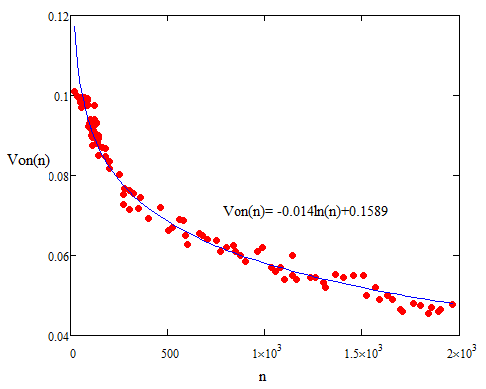
\includegraphics[width=0.77\textwidth]{amg3m.png}
    \label{amg3m}
  }
  \subfigure[]{
    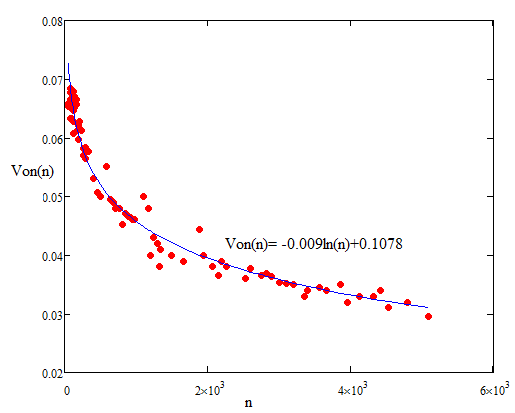
\includegraphics[width=0.77\textwidth]{10kp.png}
    \label{10kp}
  }
  \caption{
    Изменение скорости режущего инструмента
    на рабочем ходу: \\
    {\it а} -- АМг3М, $\Delta$ = 1 мм ($n \in \overline{10,2000}$); \\
    {\it б} -- Ст10кп, $\Delta$ = 3 мм ($n \in \overline{10,5000}$)
  }
  \label{amg3m+10kp}
\end{figure}

\item
Заданная в УП скорость
$V_{on}$
совпадает с фактической средней скоростью
при достижении числа кадров некоторого порогового значения $N$.
Когда количество кадров в УП меньше порогового значения $n<N$,
то фактическая скорость выше заданной,
а при увеличении числа кадров больше порогового $n>N$
-- может существенно снижаться
(в проведенных экспериментах снижение средней
фактической скорости режущего инструмента по сравнению
с заданным в УП значением доходило до 70 \%).

\item
Пороговое значение различно для разных марок материала и толщин.

\end{enumerate}

Для изложения результатов вычислительных экспериментов
введем следующие обозначения:
пусть
$n$ -- число кадров в УП,
$V_\text{факт}$ -- фактическая средняя скорость режущего инструмента при заданной скорости $V_{on}$,
$N$~-- число кадров (пороговое значение), для которого $V_\text{факт}=V_{on}$;
$\sum \varepsilon_n^2$ -- сумма квадратов отклонений исходных значений
скорости режущего инструмента и значений аппроксимирующей функции $V_{on}(n)$
в этих точках.

При аппроксимации точечных графиков
зависимости фактической скорости
$V_\text{факт}$
от числа кадров $n$
в УП аппроксимирующими кривыми в
{\it Mathcad}
для всех значений исследуемых марок материала и толщин материала было установлено,
что сходимость
$\sum \varepsilon_n^2 \to 0$
достигается при аппроксимации экспериментальных данных логарифмической функцией.

Аналогичные результаты были получены для материала
АМг3М $\Delta$~=~2--5 мм
и 10кп $\Delta$ = 1--10 мм.
Обобщенные результаты для всех исследованных марок материала и толщин
приведены в табл.~\ref{v-formulae}.

При использовании материала других марок
необходимо проведение дополнительных исследований
либо использование имеющихся данных по материалу
с близкими физическими свойствами.

Рассмотрим пример оптимизации времени резки
$T_{cut}$
(\ref{cutting-time})
при резке 15 фигурных заготовок
(материал АМг3М, $\Delta$ = 1 мм).
Раскройная карта
(рис.~\ref{amg-cutting+optimal})
содержит 15 заготовок двух типоразмеров,
при этом количество граничных контуров заготовок равно 19.
Каждый контур вырезается с помощью резки
<<по замкнутому контуру>>.
С целью сокращения множества допустимых решений
задачи множество возможных точек врезки было
ограничено конечным множеством
(задача $GTSP$),
состоящим из 55 точек
(обозначены маленькими квадратиками;
соответствующие точки выключения инструмента обозначены крестиками).
Для решения задачи использован точный алгоритм на основе ДП.
УП резки для данного примера содержат 120~команд или кадров
(т. е. $n=120$),
которые включают команды перемещения инструмента
для резки контуров
(с учетом разбиения каждого контура на несколько геометрических примитивов)
на рабочем ходу,
команды перемещения инструмента на холостом ходу
и ряд технологических команд.
Скорость рабочего хода инструмента, заданная в УП,
$V_{on}=0,1$ м/с.

\begin{table}[H]
  \caption{
    Обобщенная таблица формул
    для вычисления рабочей скорости инструмента
    на~лазерном комплексе
    {\it ByStar 3015}
    }
  \label{v-formulae}
  \centering
  \begin{tabular}{l|l|l}
    \hline
    Материал & Толщина, мм & Формула расчета $V_{on}$ \\
    \hline
    \multicolumn{3}{c}{$n\in\overline{10,5000}$} \\
    10кп & 1 & $V_{on} = -0,024 \ln n+0,245$ \\
    10кп & 2 & $V_{on} = -0,015 \ln n+0,1686$ \\
    10кп & 3 & $V_{on} = -0,009 \ln n+0,1078$ \\
    10кп & 3,5 & $V_{on} = -0,006 \ln n+0,0756$ \\
    10кп & 4 & $V_{on} = -0,006 \ln n+0,0709$ \\
    10кп & 8 & $V_{on} = -0,003 \ln n+0,0442$ \\
    10кп & 10 & $V_{on} = -0,002 \ln n+0,0365$ \\
    \multicolumn{3}{c}{$n\in\overline{10,2000}$} \\
    АМг3М & 1 & $V_{on} = -0,014 \ln n+0,1589$ \\
    АМг3М & 1,5 & $V_{on} = -0,001 \ln n+0,011$ \\
    АМг3М & 3 & $V_{on} = -0,004 \ln n+0,0672$ \\
    АМг3М & 4 & $V_{on} = -0,001 \ln n+0,0301$ \\
    АМг3М & 5 & $V_{on} = -6\cdot 10^{-4} \ln n+0,0177$ \\
    \hline
  \end{tabular}
\end{table}

На рис. \ref{amg-cutting+optimal}, {\it а}
показан маршрут резки
(перемещение инструмента на холостом ходу показано стрелками),
для которого значение целевой функции
$T_{cut}$ (\ref{cutting-time})
при
$V_{on}=0,1$ м/с
составляет
$T_{cut}=126,27$ с.
Однако фактическое время резки по управляющей программе,
составленной для этого маршрута,
оказалось (как и ожидалось)
значительно больше,
поскольку число кадров в программе ($n=120$)
значительно больше порогового значения $N=70$
для материала
АМг3М
$\Delta$ = 1 мм.

При использовании значения
$V_{on}=-0,014 \ln n + 0,1589$
(табл.~\ref{v-formulae})
в целевой функции (\ref{cutting-time})
оптимизационная процедура ДП
дает другое оптимальное решение задачи,
которое показано на рис.~\ref{amg-cutting+optimal}, {\it б}.
Тогда среднее фактическое значение
рабочей скорости инструмента при $n=120$
составило
$V_{on}=0,0919$ м/с.
В свою очередь,
для оптимального маршрута резки значение времени резки составило
$T_{cut}=141,38$ с.

\begin{figure}[H]
  \centering
  \subfigure[]{
    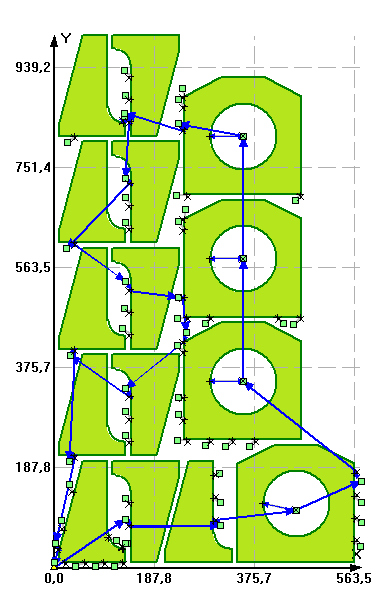
\includegraphics[width=0.45\textwidth]{amg-cutting.png}
    \label{amg-cutting}
  }
  \subfigure[]{
    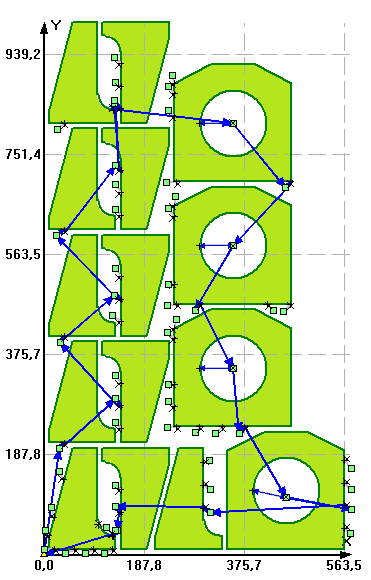
\includegraphics[width=0.45\textwidth]{amg-optimal.png}
    \label{amg-optimal}
  }
  \caption{
    Раскройная карта и оптимальный по времени маршрут
    перемещения режущего инструмента для 15 заготовок
    (материал АМг3М, $\Delta$ = 1 мм): \\
    {\it а} -- $V_{on}=const=0,1$ м/с; \\
    {\it б} -- $V_{on}=-0,014 \ln n + 0,1589$
  }
  \label{amg-cutting+optimal}
\end{figure}

Таким образом,
точное вычисление целевой функции для
данного примера обеспечило не только
точное вычисление значения экстремума
целевой функции, но и другой (правильный)
результат поиска оптимального маршрута резки,
полученный  с учетом числа кадров УП.

Этот пример иллюстрирует необходимость
получения таблиц типа табл.~\ref{v-formulae}
при решении конкретных оптимизационных задач
маршрутизации инструмента машин листовой резки с ЧПУ.
